\begin{figure}[h!]
	\caption[Zusammenhang Wellenlänge - Wellenzahl]{Dargestellt ist der Zusammenhang zwischen der Wellenlänge $\lambda$ und der Wellenzahl $n$. Da die Phase alle $2\pi$ den gleichen Wert annimmt, wird mit dem Faktor $n$ ein vielfaches der Wellenlänge aufaddiert. Dadurch erhält man die Entfernung zu dem Tag.}
	\label{fig:wavenumber_wavelength}
	\begin{gnuplot} % aufrufen des Befehls und anschließende eingabe der Gnuplot Befehle
		set terminal epslatex color % WICHTIG: diese Zeile teilt Gnuplot 
		                            % mit das die Ausgabe in Latex umgeleitet werden soll
		set nokey % ab hier folgt üblicher Gnuplot Code
		set parametric
		set hidden3d
		set view 45,60
		set isosamples 200,15
		splot [-3*pi:3*pi][-pi:pi] cos(u)*cos(v)+3*cos(u)*(1.5+sin(u*5/3)/2),\
		sin(u)*cos(v)+3*sin(u)*(1.5+sin(u*5/3)/2), sin(v)+2*cos(u*5/3)
	\end{gnuplot}
\end{figure}
%%
%% usage: {alpha}{phasedifferenceUI}{voltage}{current}{Ualpha}{Ialpha}
%% resistor
\ZeigerdiagrammText{110}{-80}{2}{2}
%
%\begin{figure} [h]
%\centering
%        
%         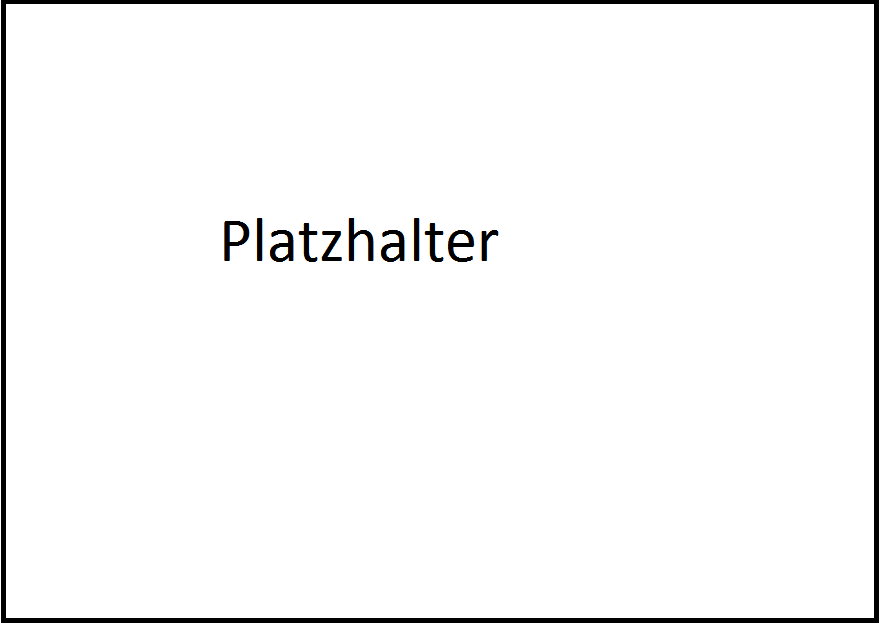
\includegraphics[width=\textwidth]{img/00_placeholder.png}
%%      
%\end{figure}

Aus der Abbildung~\ref{fig:wavenumber_wavelength} lässt sich folgender Zusammenhang ableiten.
%
\begin{equation}
\label{eq:Phase_Wavenumber}
	d(\Theta, n)=\lambda(\sfrac{\Theta}{2\pi}+n)
\end{equation}